\documentclass[12pt, letterpaper, parskip = full]{article}
\usepackage[mmddyyyy]{datetime}

\usepackage[utf8]{inputenc}
\usepackage{amsmath}
\usepackage{mathpazo}
\usepackage{eulervm}
\usepackage[skip=10pt plus1pt]{parskip}

\usepackage[margin=1in]{geometry}
\linespread{1.20}
\usepackage{enumerate}
\usepackage{enumitem}
\usepackage{listings}
\usepackage[T1]{fontenc}
\usepackage{amsfonts}
\usepackage{amssymb}
\usepackage{amsthm}
\usepackage{multirow,array}
\usepackage{graphicx}
\usepackage{physics}
\usepackage{bm}
\usepackage{tikz}
\usepackage{breqn}
\usepackage[longnamesfirst]{natbib}
\usepackage{comment}
\usepackage{setspace}
\usepackage{hyperref}
\usepackage{accents}
\usepackage{graphicx}

\graphicspath{{Images/}}
\setlength{\parindent}{0pt}

\newtheorem{theorem}{Theorem}
\newtheorem{corollary}{Corollary}
\newtheorem{lemma}{Lemma}
\newtheorem{definition}{Definition}
\newtheorem{axiom}{Axiom}
\newcommand{\e}{\mathrm{e}}
\newcommand{\Var}{\mathrm{Var}}
\newcommand{\Ex}[1]{\mathbb{E}\left[#1\right]}
\renewcommand{\Pr}[1]{\mathbb{P}(#1)}
\newcommand{\plim}{\mathrm{plim}}
\newcommand{\pc}[1]{\frac{\dot{#1}(t)}{#1(t)}}
\renewcommand\qedsymbol{$\blacksquare$}
\newcommand{\ubar}[1]{\underaccent{\bar}{#1}}

\title{Homework 2 \\ Macroeconomic Theory I}
\author{Alejandro Flores-Brown}

\begin{document}
	
	\maketitle

    \section{Steady State}

    We are given the equilibrium condition in steady-state already; that means the only remaining step is to solve it by bisection. Fundamentally this is the same problem as Part C of Homework 1, so we can reuse similar code with different parameters, with the only change being to write a function to test the free-entry condition. The steady state is given to three decimal places as

    \begin{center}
	\begin{tabular}{|c|c|c|c|c|c|c|c|}
		\hline
		\(\theta^*\) & \(\lambda_w\) & \(\lambda_f\) & \(w^*\) & \(u^*\) & \(S\) & \(J\) & \(\text{Free Entry condition}\) \\
		\hline
		\(0.723\) & \(0.451\) & \(0.623\) & \(0.971\) & \(0.042\) & \(2.416\) & \(1.208\) & \(0.000\)\\
		\hline
	\end{tabular}
	\end{center}

    With the previous code, it is also easy to plot unemployment versus b. This yields the expected result that raising the value of unemployment directly leads to less people being employed, as the surplus gained from working is smaller.

    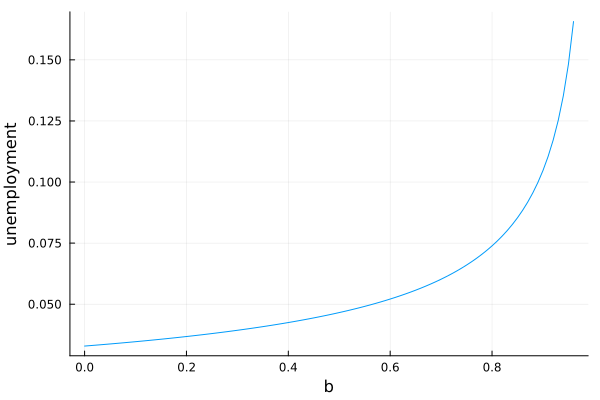
\includegraphics[scale=0.4]{u_vs_b.png}

    \section{The Shimer exercise in steady-state}

    \subsection{}

    We first must find a new \(\gamma', b'\) pair that leaves the steady-state unchanged. This is relatively easy to do numerically: we fix \(\gamma'\), then use bisection to solve for the zero of \(\theta' - \theta^*\), where \(\theta'\) is the market tightness of the new steady-state and \(\theta^*\) is the old market tightness. Concretely, this gives

    \begin{center}
	\begin{tabular}{|c|c|c|c|c|}
		\hline
		\(\gamma\) & \(\theta\) & \(u\) & \(b\) & \(\epsilon_{\theta z}\) \\
		\hline
		\(0.05\) & \(0.723\) & \(0.0.043\) & \(0.941\) & \(22.859\) \\
		\hline
	\end{tabular}
	\end{center}

    We see from this exercise that a very high level of \(b\) is still required to make the elasticity match the data even after shrinking the worker's bargaining power by a factor of \(10\). We can see this more clearly if we plot the elasticity with respect to the level of \(b\):

    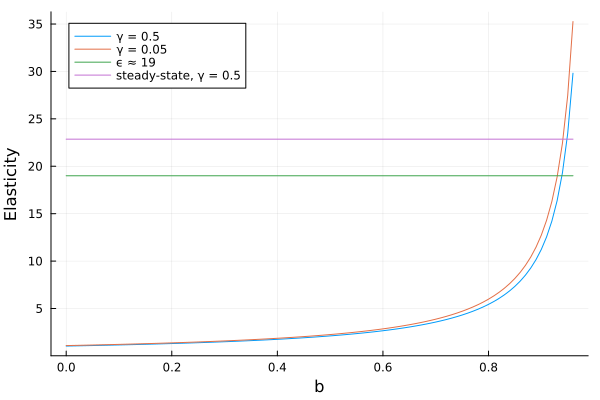
\includegraphics[scale = 0.75]{elasticities.png}

    The larger value of \(\gamma\) barely makes a difference; large elasticities require a very high \(b\) in both calibrations.

    \subsection{}

    I compute \(\frac{du}{d \ln(b)}\) as a numerical derivative. The two functions, along with the bound \(\epsilon = 0.3\), are plotted here.

    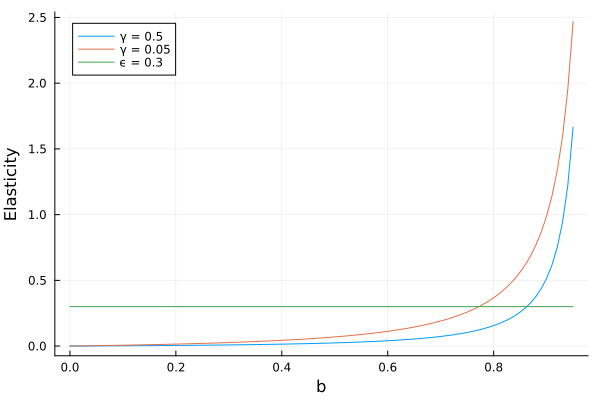
\includegraphics[scale=0.75]{belasticities.png}

    The bound displayed on this graph is overly generous since the computed elasticity should be the effect of a \(1\%\) increase in unemployment benefits, but the implication remains the same: the high-\(b\), low-\(\gamma\) calibration does not survive the data. The bound suggests an absolute maximum of \(b\) less than \(0.8\), not consistent with the computed \(b = 0.941\). The high-\(b\) calibration attempts to make the elasticity with response to productivity high by shrinking the surplus to almost nothing, but this also makes everything else overly responsive because a small surplus means the response to \emph{any} change is amplified.

    \section{The fully stochastic case}

    \subsection{}

    It is straightforward to generate the time series. So that I have something concrete to show for this section, I plot the simulated values of \(z\) below:

    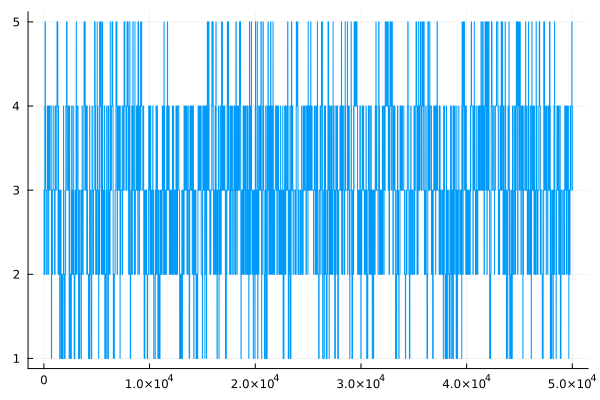
\includegraphics[scale = 0.4]{zs_plot.png}

    \subsection{}

    Simulating the model produces the following moment table:

    \begin{center}
	\begin{tabular}{|c|c|c|c|c|c|c|}
		\hline
		\(sd(\ln(z))\) & \(sd(\ln(\theta))\) & \(sd(\ln(u))\) & \(sd(\ln(w))\) & \(\frac{sd(\ln(\theta))}{sd(\ln(z))}\) & \(\frac{sd(\ln(w))}{sd(\ln(z))}\) & \(\rho(\ln(u), \ln(v))\) \\
		\hline
		\(0.384\) & \(0.036\) & \(0.016\) & \(0.025\) & \(5.612\) & \(0.064\) & \(-0.782\) \\
		\hline
	\end{tabular}
	\end{center}

    The simulated elasticity, \(\frac{sd(\ln(\theta))}{sd(\ln(z))} = 5.612\), is large, much larger than the \(\epsilon_{\theta z} = 1.751\) of our initial calibration! However, it is still not large enough to match the data in this calibration. The correlation between unemployment and vacancies is also a bit less than in the data, but the large size and negative sign is correct so this should not matter too much for the performance of the model.

    \subsection{}

    We now simulate the rigid-wage economy. A quick computation suggests that we are expecting a rigid elasticity around \(69\). We simulate and report a moment table below; the moments are the same as in the previous part minus the wage-dependent moments, since wages are fixed.

    \begin{center}
	\begin{tabular}{|c|c|c|c|c|}
		\hline
		\(sd(\ln(z))\) & \(sd(\ln(\theta))\) & \(sd(\ln(u))\)  & \(\frac{sd(\ln(\theta))}{sd(\ln(z))}\)  & \(\rho(\ln(u), \ln(v))\) \\
		\hline
		\(0.384\) & \(2.155\) & \(0.605\) & \(5.612\) & \(-0.782\) \\
		\hline
	\end{tabular}
	\end{center}

    The ratio is much smaller than the very large predicted elasticity, so there may be some error here. Regardless, the rest of the moments point to the problems expected from the question statement --- the variance of \(\theta\) and \(u\) are several orders of magnitude larger than in the previous model! These huge variances are created because most of the variation in the model is being delivered by the states where the surplus is negative: because wages are now fully rigid, the only major changes are delivered during deep recessions, when very low productivity drives \(w\) outside the bargaining set. These only occur about \(5.9\%\) of the time in this simulation, so a very small number of observations is being forced to drive the entire model! This experiment shows that a fully rigid wage norm will not accurately reproduce the data; it produces too-deep recessions during bad times and does not give enough variation during good times.



\end{document}